\begin{frame}[c]{}

\centering
\huge
Lecture 4:\\
Meta-Learning
\end{frame}
%----------------------------------------------------------------------
\begin{frame}[c]{Where are we? The big picture}

\begin{itemize}
	\item Introduction
	\item Background
	\begin{itemize}
		\item Design spaces in ML
		\item Evaluation and visualization
	\end{itemize}
	\item[$\to$] Hyperparameter optimization (HPO)
	\begin{itemize}
		\item Bayesian optimization
		\item Other black-box techniques
		\item Speeding up HPO with multi-fidelity optimization
	\end{itemize}
	\item Pentecost (Holiday) -- no lecture
	\item Architecture search I + II
	\item[$\to$] Meta-Learning
	\item Learning to learn $\&$ optimize
	\item Beyond AutoML: algorithm configuration and control
	\item Project announcement and closing
\end{itemize}

\end{frame}
%----------------------------------------------------------------------

%----------------------------------------------------------------------
\begin{frame}[c]{Learning Goals}

After this lecture, you will be able to \ldots

\begin{itemize}
	\item ...
\end{itemize}

\end{frame}
%-----------------------------------------------------------------------
%----------------------------------------------------------------------
\begin{frame}[c]{Further Material}

There were two great tutorials on meta-learning recently:

\begin{itemize}
	\item NeurIPS'18: Frank Hutter and Joaquin Vanschoren
	"Automatic Machine Learning (AutoML): A Tutorial"
	\url{https://videoken.com/embed/5A4xbv5nd8c}
	\item ICML'19: Chelsea Finn and Sergey Levine on\\
	"Meta-Learning: from Few-Short Learning to Rapid Reinforcement Learning"\\
	\url{https://www.facebook.com/icml.imls/videos/400619163874853/}
\end{itemize}

\begin{itemize}
	\item Strong recommendation to watch both tutorials
	\item We can't cover all the stuff today
	\item Parts of the material used today was inspired by these tutorials
\end{itemize}


\end{frame}
%-----------------------------------------------------------------------
\section{Meta-Learning}
%----------------------------------------------------------------------
\begin{frame}[c]{The Idea of Meta-Learning}

\begin{itemize}
	\item Learning essential never stops
	\begin{itemize}
		\item We learn several models on the same task (e.g., dataset)
		\item We learn models on new tasks
	\end{itemize}
    \pause
    \item Learning is often done from scratch
    \item[$\leadsto$] We humans don't start from scratch all the time,
    but we learned how to learn!
\end{itemize}

\bigskip

\begin{tikzpicture}

	\node (task1) [data, text width=6em] {Task~1};
	\node (learn1) [activity, below of=task1, text width=6em] {Learning};
	\node (models1) [activity, below of=learn1, text width=6em] {Models};
	\node (perf1) [data, below of=models1, text width=6em] {Performance};
	
	\node (task2) [data, right of=task1, node distance=4.5cm, text width=6em] {Task~2};
	\node (learn2) [activity, below of=task2, text width=6em] {Learning};
	\node (models2) [activity, below of=learn2, text width=6em] {Models};
	\node (perf2) [data, below of=models2, text width=6em] {Performance};
	
	\node (task3) [data, right of=task2, node distance=4.5cm, text width=6em] {Task~3};
	\node (learn3) [activity, below of=task3, text width=6em] {Learning};
	\node (models3) [activity, below of=learn3, text width=6em] {Models};
	\node (perf3) [data, below of=models3, text width=6em] {Performance};
	
	\draw[myarrow] (task1) -- (learn1);
	\draw[myarrow] (learn1) -- (task1);
	\draw[myarrow] (learn1) -- (models1);
	\draw[myarrow] (models1) -- (perf1);
	
	\draw[myarrow] (task2) -- (learn2);
	\draw[myarrow] (learn2) -- (task2);
	\draw[myarrow] (learn2) -- (models2);
	\draw[myarrow] (models2) -- (perf2);
	
	\draw[myarrow] (task3) -- (learn3);
	\draw[myarrow] (learn3) -- (task3);
	\draw[myarrow] (learn3) -- (models3);
	\draw[myarrow] (models3) -- (perf3);
	
	\draw[myarrow] (learn1) -- node[above] {Meta-Learn} (learn2);
	\draw[myarrow] (learn2) -- node[above] {Meta-Learn} (learn3);	
\end{tikzpicture}

\end{frame}
%-----------------------------------------------------------------------
\begin{frame}[c]{Example for Human Meta-Learning}

\begin{columns}
	\column{0.18\textwidth}
	Braque
	\centering
	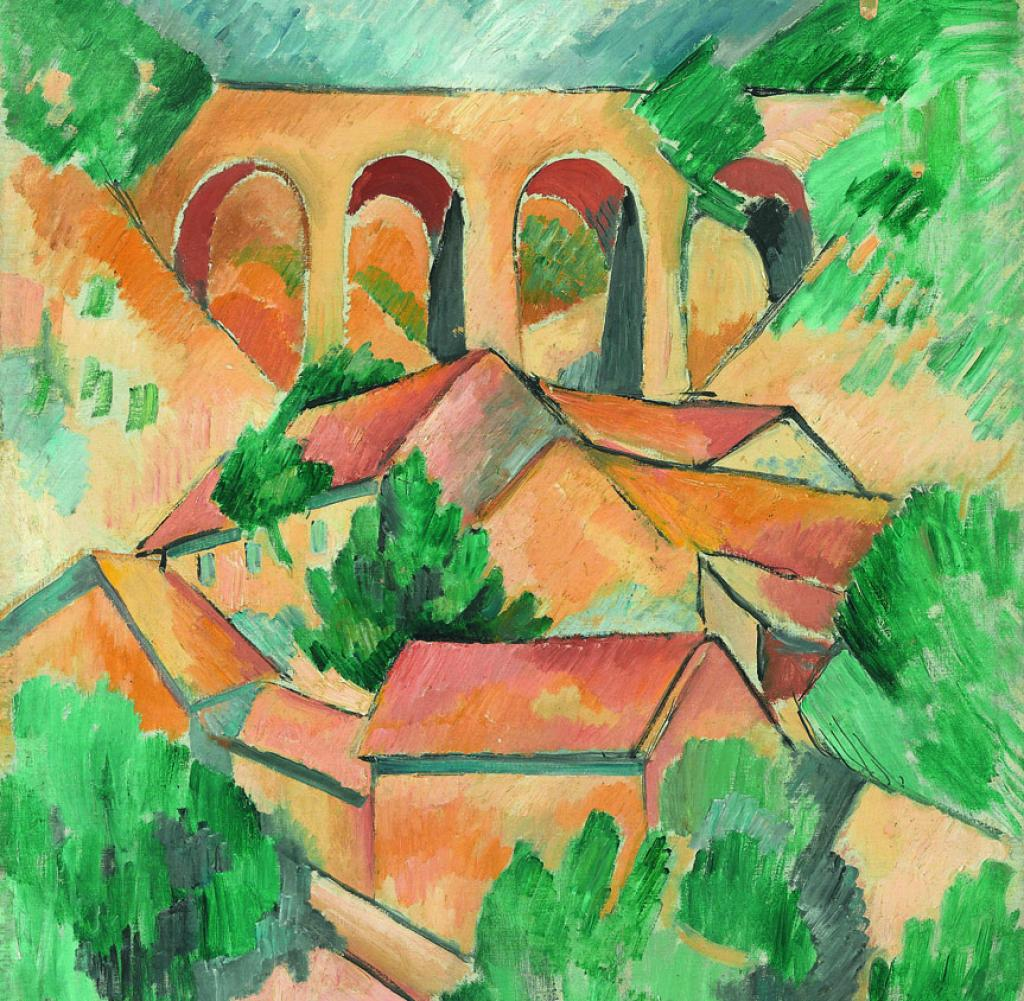
\includegraphics[width=1.0\textwidth]{images/braque1.jpg}
	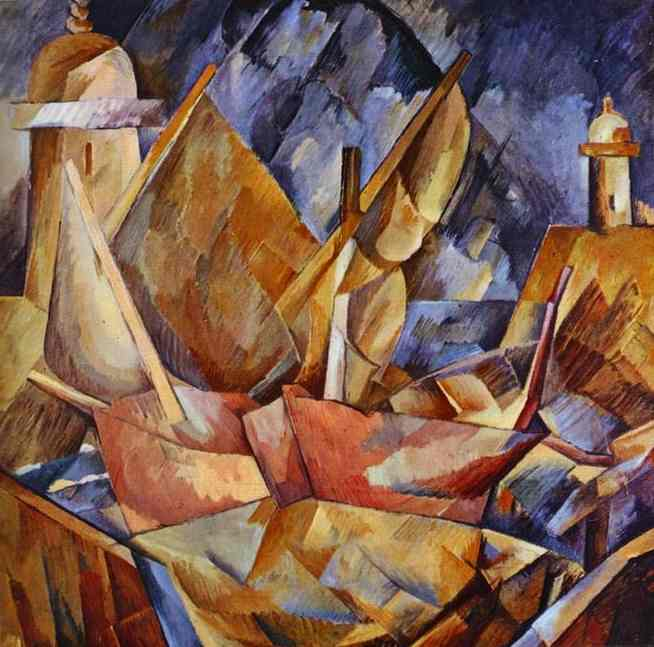
\includegraphics[width=1.0\textwidth]{images/braque2.jpeg}
	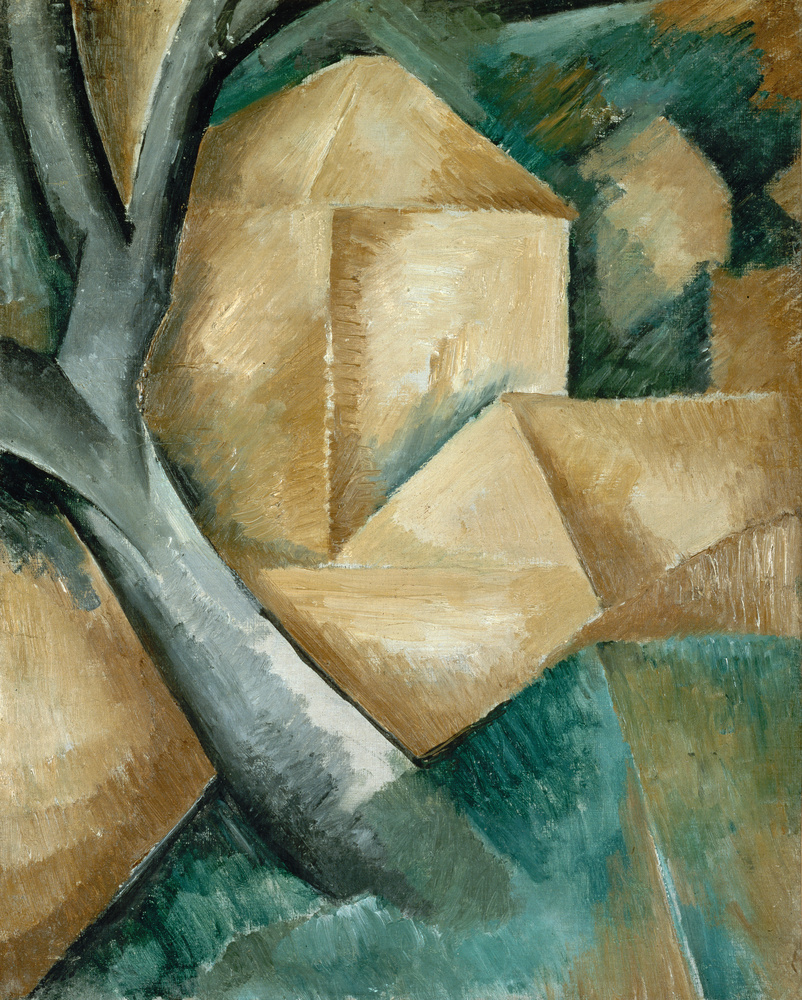
\includegraphics[width=1.0\textwidth]{images/braque3.jpg}
	\column{0.258\textwidth}
	Cezanne
	\centering
	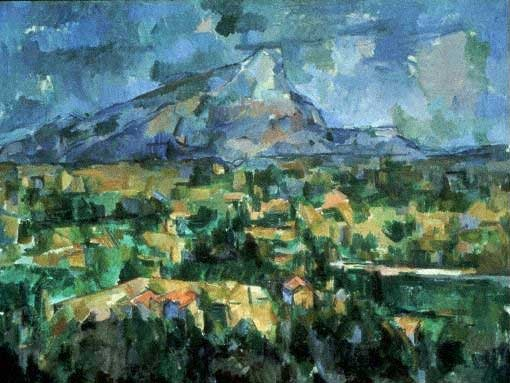
\includegraphics[width=1.0\textwidth]{images/cezanne1.jpg}
	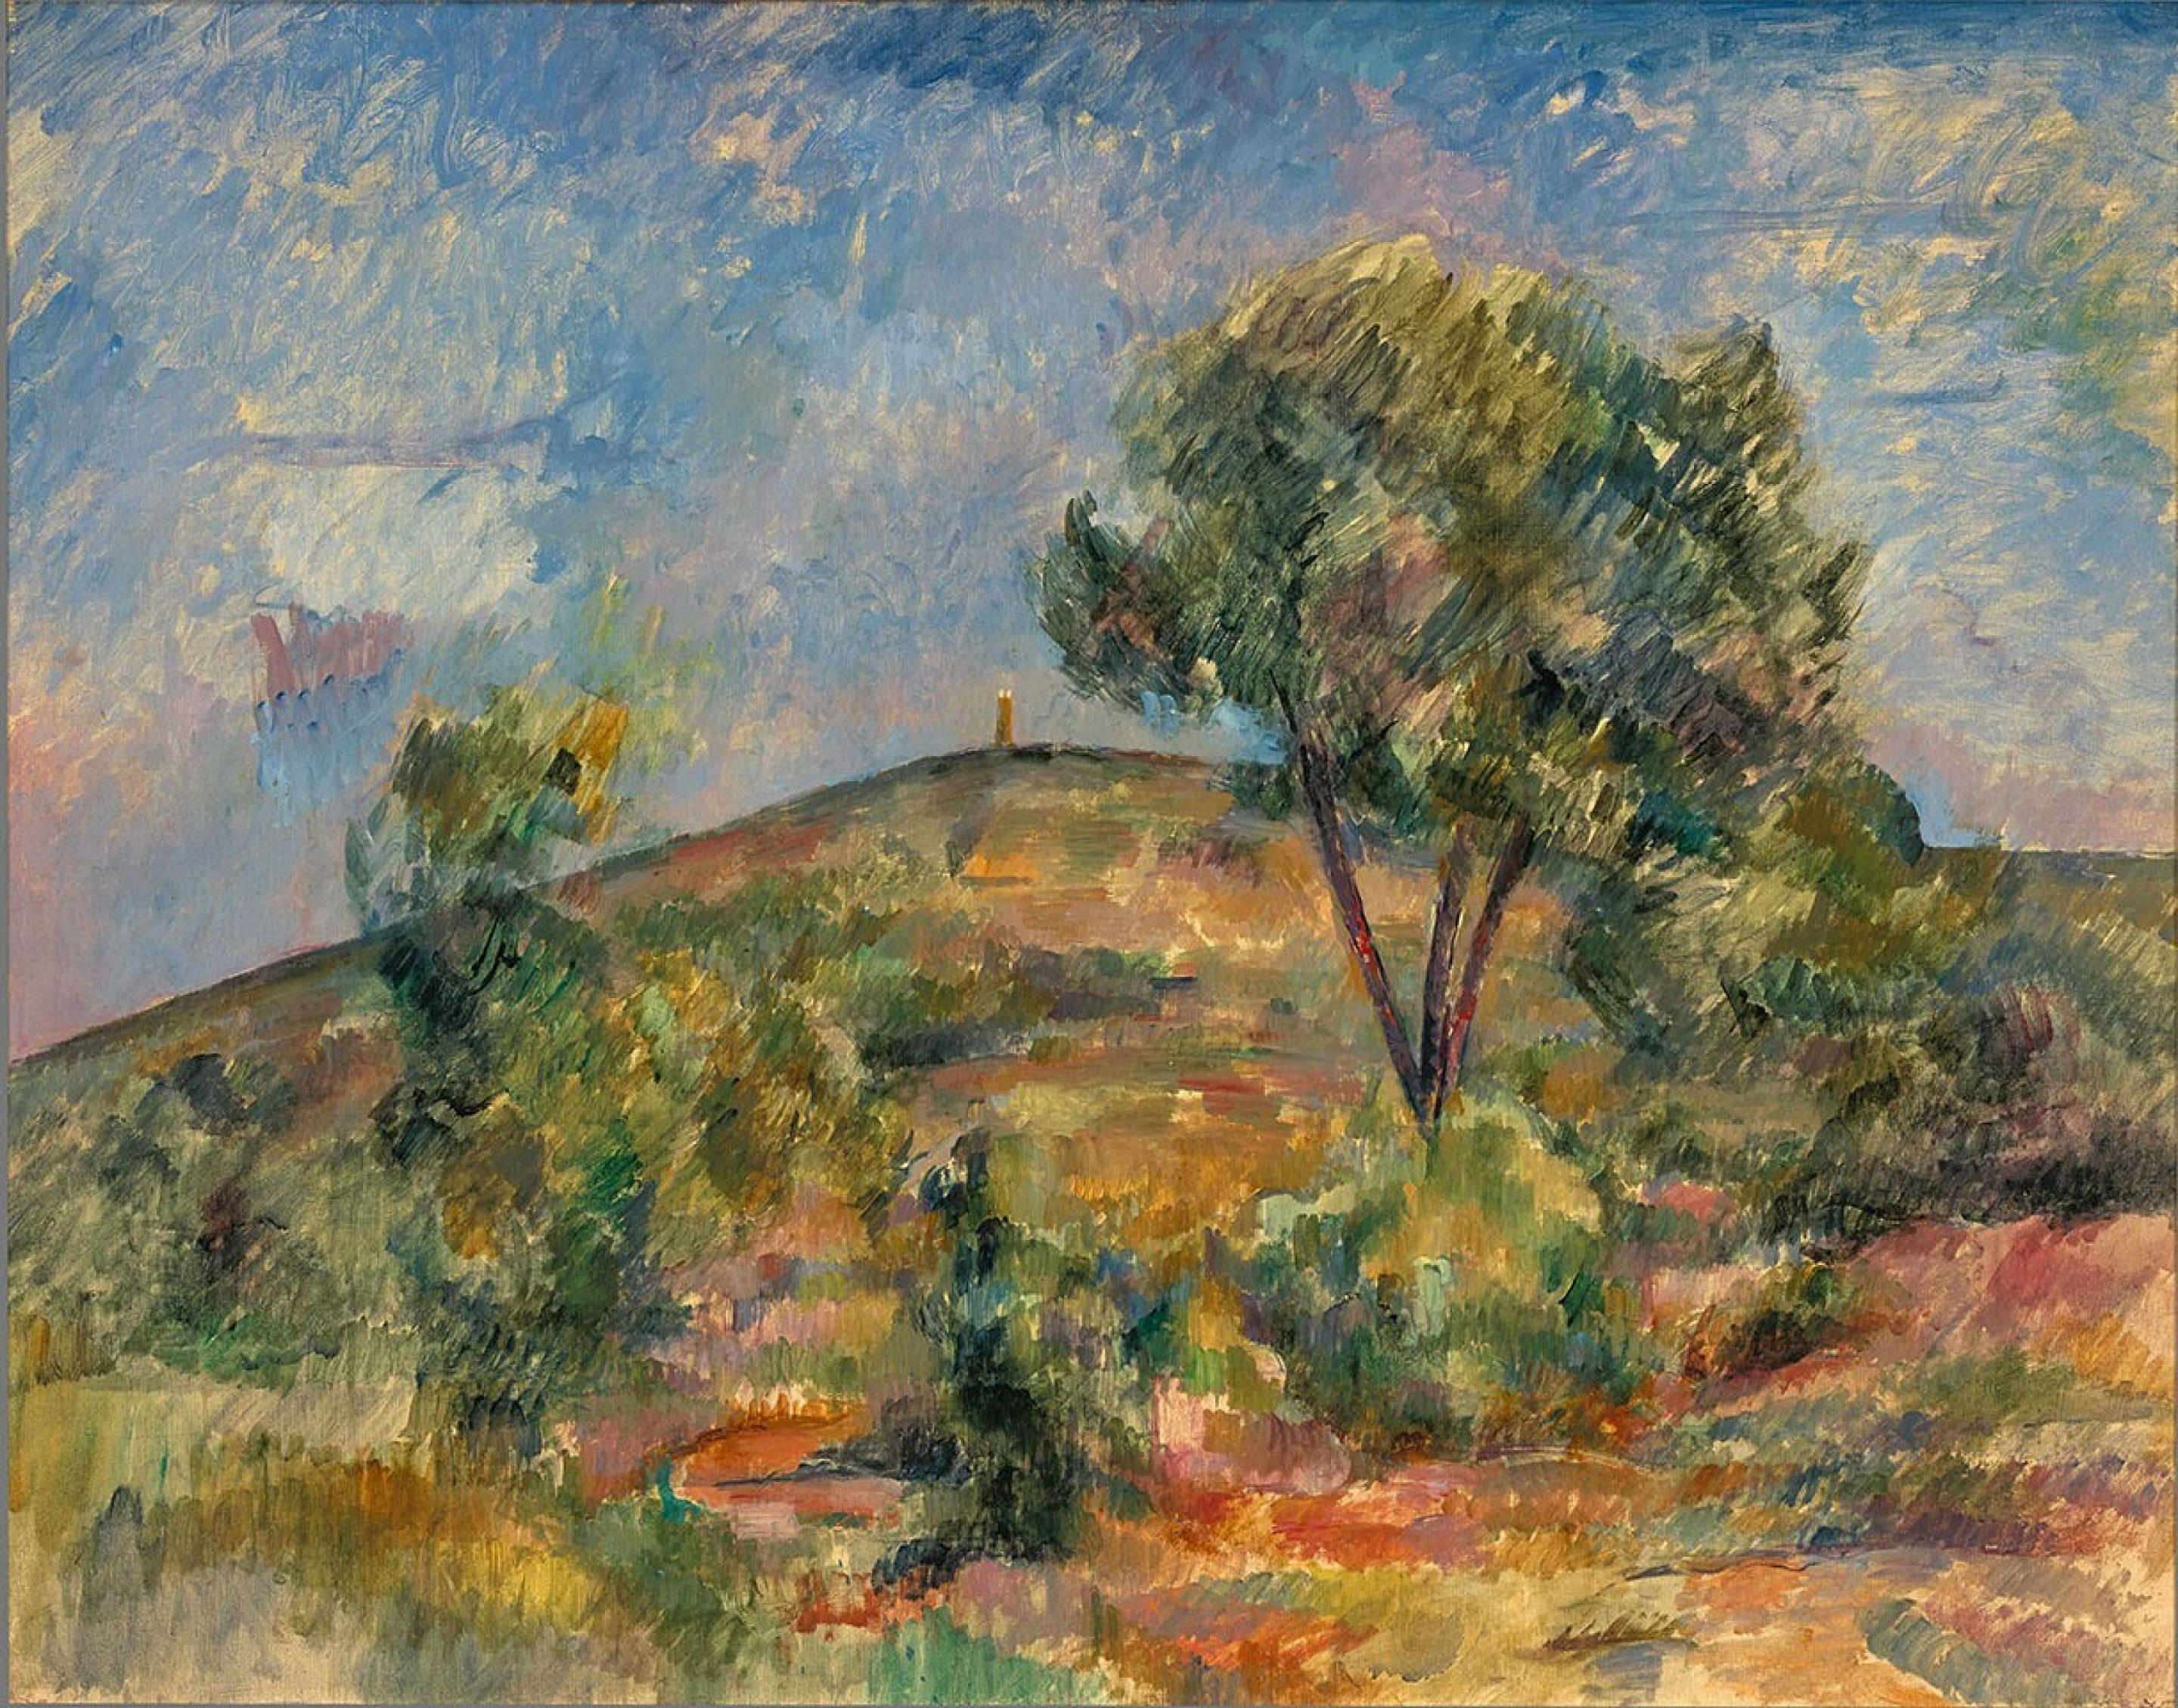
\includegraphics[width=1.0\textwidth]{images/cezanne2.jpg}
	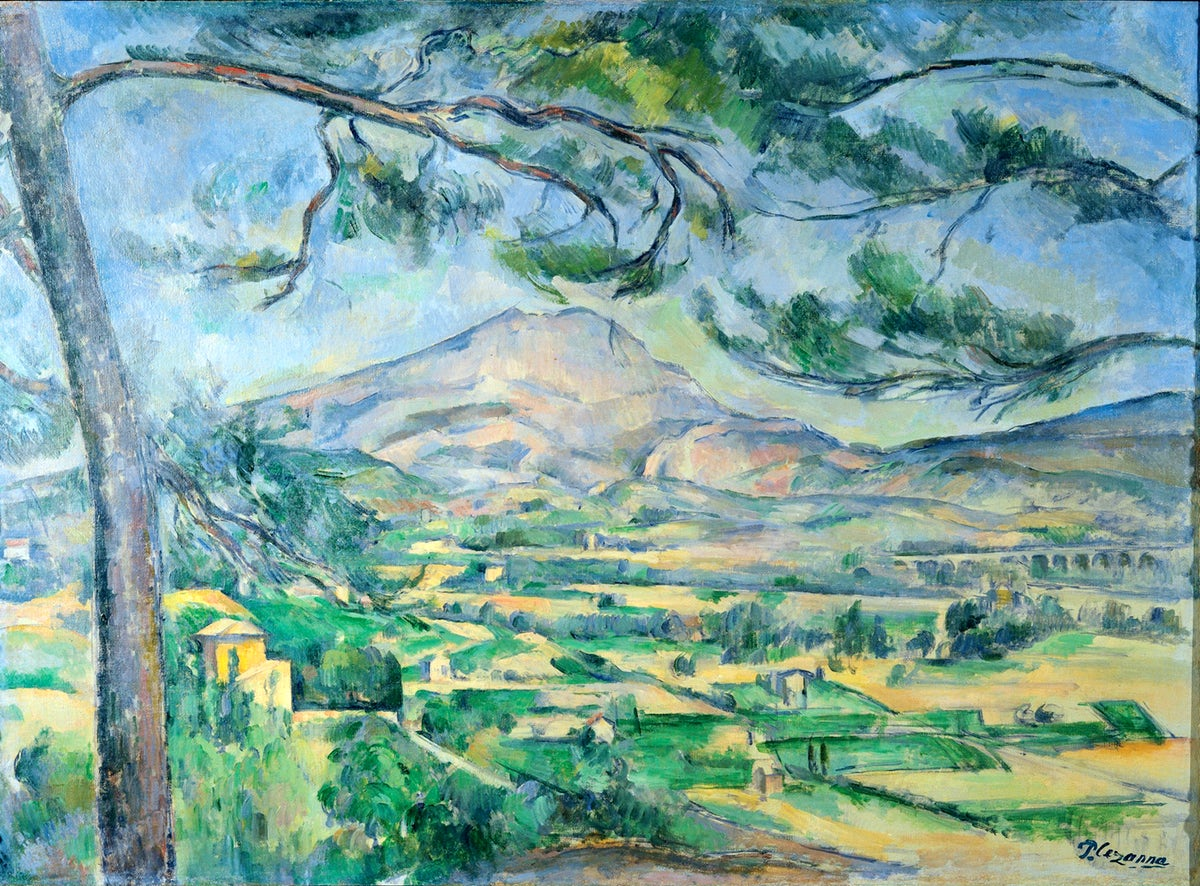
\includegraphics[width=1.0\textwidth]{images/cezanne3.jpg}
	\column{0.3\textwidth}
	\centering
	Who painted that?
	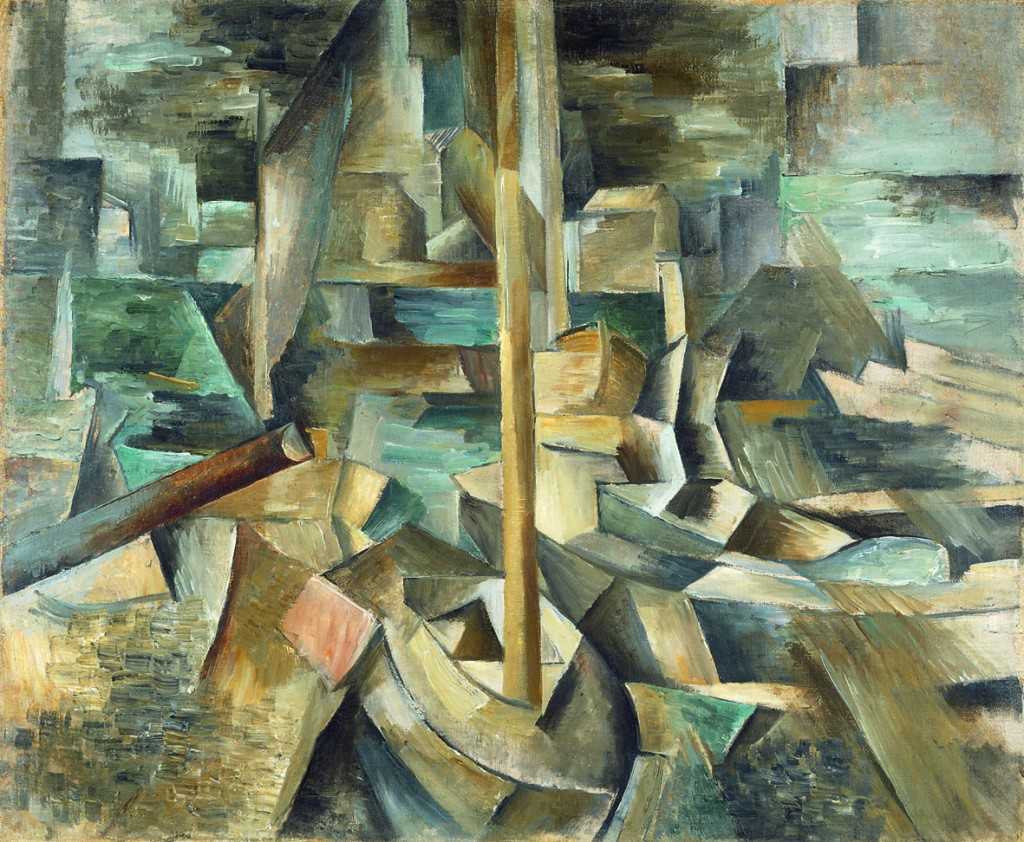
\includegraphics[width=1.0\textwidth]{images/Braque4.jpg}
	
	\pause
	Most likely most of you can identify the painter correctly, 
	although I presented only three pictures of each.
\end{columns}

\end{frame}
%-----------------------------------------------------------------------
%-----------------------------------------------------------------------
\begin{frame}[c]{Recap Supervised Learning}

Dataset:
\begin{equation}
\dataset = \{(x_1, y_1), \ldots, (x_k, y_k) \}
\end{equation}

\bigskip
\pause

Learning a model $\phi$ (e.g., weights of a neural network):
\begin{eqnarray}
\argmax_{\phi} \log p(\phi|\dataset)\\
= \argmax_{\phi} \log p(\dataset | \phi) + \log p(\phi) \\
= \argmax_{\phi} \sum_i \log p(y_i | x_i, \phi) + \log p(\phi)
\end{eqnarray}

Challenge:
\begin{itemize}
	\item Learning starts from scratch\\
	(e.g., we initially have no clue what could a good $\phi$)
	\item we might only have very few examples in $\dataset$\\
	(i.e., $k$ is small)
\end{itemize}

\end{frame}
%-----------------------------------------------------------------------
%-----------------------------------------------------------------------
\begin{frame}[c]{The Meta Learning Problem}

Dataset:
\begin{equation}
\dataset = \{(x_1, y_1), \ldots, (x_k, y_k) \}
\end{equation}
Set of datasets (meta-datasets):
\begin{equation}
\dataset_{\text{meta-train}} = \{\mathcal{D}_1, \ldots, \mathcal{D}_n, \}
\end{equation}

\pause
Can we include these meta-datasets to improve learning on $\dataset$?
\begin{equation}
\argmax_{\phi} \log p(\phi|\dataset, \dataset_{\text{meta-train}})
\end{equation}

\pause
\medskip

\alert{Idea:} Instead of keeping $\dataset_{\text{meta-train}}$ forever, we want to distill the knowledge into \alert{meta-parameters $\theta$}: $p(\theta|\dataset_{\text{meta-train}})$
 

\end{frame}
%-----------------------------------------------------------------------
%-----------------------------------------------------------------------
\begin{frame}[c]{The Meta Learning Problem}

So, we want to learn:
\begin{eqnarray}
\argmax_{\phi} \log p(\phi|\dataset, \dataset_{\text{meta-train}}) \\
= \argmax_{\phi} \log \int_{\Theta} p(\phi \mid \dataset, \theta) p(\theta \mid \dataset_{\text{meta-train}}) d\theta\\
\approx \argmax_{\phi} \log p(\phi | \dataset, \theta^*) + \log p(\theta^* | \dataset_{\text{meta-train}})\\
= \argmax_{\phi} \log p(\phi | \dataset, \theta^*)
\end{eqnarray}

The meta-learning problem is:
\begin{equation}
\argmax_{\theta} \log p(\theta | \dataset_{\text{meta-train}})
\end{equation}



\end{frame}
%-----------------------------------------------------------------------
%-----------------------------------------------------------------------
\section{Algorithm Selection}
%----------------------------------------------------------------------
\begin{frame}[c]{XXX}



\end{frame}
%-----------------------------------------------------------------------
%-----------------------------------------------------------------------
\section{HPO Warmstarting}
%----------------------------------------------------------------------
\begin{frame}[c]{XXX}



\end{frame}
%-----------------------------------------------------------------------
%-----------------------------------------------------------------------
\section{Few Shot Learning}
%----------------------------------------------------------------------
\begin{frame}[c]{XXX}



\end{frame}
%-----------------------------------------------------------------------

%----------------------------------------------------------------------
\begin{frame}[c]{Learning Goals}

After this lecture, you are able to \ldots

\begin{itemize}
	\item ...
\end{itemize}
\end{frame}
%-----------------------------------------------------------------------

%----------------------------------------------------------------------
\begin{frame}[c]{Literature [These are links]}

\begin{itemize}
	\item \lit{\href{}{}}	
\end{itemize}

\end{frame}
%----------------------------------------------------------------------


